\subsection{Queue For Resources}

\subsubsection*{Ausgangslage}

Ein System versucht eine Überlastung zu verhindern. Es ist aber nicht mit einer Fehlerbehandlung beschäftigt sondern erhält einfach zu viele Anfragen.

\subsubsection*{Lösungsansatz}

Eine Möglichkeit wäre, nur die Anfragen zu behandeln, welche mit den freien Ressourcen behandelt werden können. Alle anderen werden verworfen. Shed Load (49) löst eine Überlastung so. Mit diesem Ansatz gibt es aber einige Probleme:
\begin{itemize}
	\item Eine Anfrage, welche sich aus mehreren kleineren Anfragen zusammensetzt, kann nicht abgeschlossen werden, weil eine Anfrage abgewiesen wurde.
	\item Wichtige Anfrage werden ohne Prüfung ignoriert (Siehe Maintenance Interface (7))
	\item Die Überlastung kann nur von kurzer Zeit sein und eine abgewiesen Anfrage könnte kurze Zeit später verarbeitet werden.
\end{itemize}

\begin{itemize}
	\item Die Queue wird zu lange, sodass sie nicht mehr verwaltet werden kann.
	\item Es stehen auch nach einer Weile nicht genügend Ressourcen für die vorderste Anfrage bereit und diese blockiert nun die Queue oder muss verworfen werden.
	\item Die Verwaltung der Queue benötigt zusätzliche Ressourcen und kann sehr ineffizient umgesetzt sein.
\end{itemize}

\subsubsection*{Schlussfolgerung}

Speichere Anfragen, die nicht direkt verarbeitet werden können, in einer Queue.

\begin{figure}[H]
	\centering
	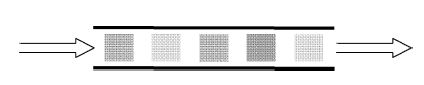
\includegraphics[width=\textwidth]{content/faulttolerance/images/QueueForResources.JPG}
	\caption{QueueForResources}
\end{figure}


\subsubsection*{Verwandte Patterns}

Queues:
\begin{itemize}
	\item FIFO (First In/First Out): Für Systemanfragen
	\item LIFO (Last In/First Out aka Stack): Für Anfragen von Benutzern. Derjenige, der als letztes die Anfrage abgesetzt hat, erhält am schnellsten Antwort. Derjenige, der als erstes eine Anfrage gestellt hat, hat wohl bereits aufgegeben.
\end{itemize}

\begin{itemize}
	\item Equitable Resource Allocation (45)
\end{itemize}


